%======================================================================
% Poznamky_4_skladani_ang_mom.pdf
%======================================================================
\section{Skládání momentu hybnosti}
\strana{AA-1}

\textbf{Opakování z minulého semestru:}

\begin{definice}[Moment hybnosti]
\kw{Moment hybnosti} \dots\ libovolný operátor (vektorový) \quad
$[\hat J_i,\hat J_j] = i\hbar\,\varepsilon_{ijk}\hat J_k$, \quad $i = x,y,z$
\end{definice}

$\Rightarrow$ spektrum $J^2, J_z$ \dots\ spol.\ vl.\ vektory $\ket{j,m,\alpha}$

\begin{minipage}{0.6\textwidth}
\begin{align*}
  J^2\ket{j,m,\alpha} &= j(j+1)\hbar^2\ket{j,m,\alpha} \\
  J_z\ket{j,m,\alpha} &= m\hbar\ket{j,m,\alpha}
\end{align*}
\end{minipage}
\begin{minipage}{0.38\textwidth}
$j = 0,\frac12,1,\frac32,\dots$ (nebo podmnožina) \\
$m = -j,-j+1,\dots,j$ \\
($\forall j$; $2j+1$ hodnot + různá degenerace)
\end{minipage}

přitom
\[
  \vzorec{\begin{aligned}
    J_+\ket{j,m} &= \sqrt{(j-m)(j+m+1)}\,\hbar\ket{j,m+1} \\
    J_-\ket{j,m} &= \sqrt{(j+m)(j-m+1)}\,\hbar\ket{j,m-1}
  \end{aligned}}
\]
\quad kde \quad $J_\pm \equiv J_x \pm iJ_y$

\begin{priklad}[příklady]
\begin{itemize}[nosep]
  \item spin $\frac12$: \quad $\hat{\vec S} = \frac{\hbar}{2}(\sigma_x,\sigma_y,\sigma_z)$ \quad
        $\leftarrow \left(\begin{pmatrix}0&1\\1&0\end{pmatrix},\begin{pmatrix}0&-i\\ i&0\end{pmatrix},\begin{pmatrix}1&0\\0&-1\end{pmatrix}\right)$
  \item orbit.\ moment: \quad
        $\hat{\vec L} = \hat{\vec x}\times\hat{\vec p} = -i\hbar\Big(y\pdv{z} - z\pdv{y},\ z\pdv{x} - x\pdv{z},\ x\pdv{y} - y\pdv{x}\Big)$
        \pozn{v originále složky zapsány v pořadí $z$, $y$, $x$ se šipkou na prohození}
\end{itemize}
\end{priklad}

\kw{Skládání systémů:} \quad $\mathcal{H} = \mathcal{H}_1\otimes\mathcal{H}_2$ \quad
\dots\ $\ket{\psi} = \ket{\phi_1}\otimes\ket{\phi_2}$ (nebo lin.\ kombinace) \\
\hspace*{6cm} báze $\ket{\phi_{mn}} = \ket{\phi_m}_1\otimes\ket{\phi_n}_2$ \\
\quad operátory \quad $\hat A_1 \to \hat A_1\otimes\hat I$ \qquad
$\hat A_1\otimes\hat I\big(\ket{\phi_1}\otimes\ket{\phi_2}\big) = \hat A_1\ket{\phi_1}\otimes\ket{\phi_2}$

částice se spinem $\frac12$: \dots\ báze $\ket{\vec Q,s} \equiv \ket{x,y,z}\otimes\ket{\pm}$ \quad \dots\ $\mathcal{H} = \mathcal{L}^2(\mathbb{R}^3)\otimes\mathbb{R}^2$

\quad vln.\ fce má teď komponenty \quad
$\psi_\pm(x,y,z) \equiv \underbrace{\bra{x,y,z}\otimes\bra{\pm}}_{\in\mathcal{H}^*}\underbrace{\ket{\psi}}_{\mathcal{H}}$

\quad tj.\ $\ket{\psi} \equiv \begin{pmatrix}\psi_+(\vec Q)\\ \psi_-(\vec Q)\end{pmatrix}$ \quad \dots\ dvoukomponentová vln.\ fce

celkový moment hybnosti \quad $\hat{\vec J} = \hat{\vec L} + \hat{\vec S} \equiv \hat{\vec L}\otimes\hat I + \hat I\otimes\hat{\vec S}$

tj.\ např.\ $J_z\ket{\psi}$ \dots\ v souřad.\ reprez.\
\[
  = -i\hbar\begin{pmatrix} x\partial_y\psi_+ - y\partial_x\psi_+ \\ x\partial_y\psi_- - y\partial_x\psi_-\end{pmatrix}
  + \frac{i\hbar}{2}\underbrace{\sigma_z\begin{pmatrix}\psi_+\\ \psi_-\end{pmatrix}}_{\begin{pmatrix}1&0\\0&-1\end{pmatrix}\begin{pmatrix}\psi_+\\ \psi_-\end{pmatrix}}
\]

v případě, že $H$ je sfér.\ sym.\ nezáv.\ na spinu \\
\dots\ místo $Q$-reprezentace \quad
$\left.\begin{aligned} &\ket{n\,l\,m}\ket{+} \\ &\ket{n\,l\,m}\ket{-}\end{aligned}\right\}$
vl.\ v.\ $H, L^2, L_z, S_z, S^2$ \ ($S^2 \hookrightarrow$ vždy $\frac34\hbar^2$) \\
\hspace*{5.8cm} $\to \ket{n,l,m,s_z}$

$\to$ ukážeme, že \sout{dob} ÚSKO je též \quad $J^2, J_z, L^2, S^2$ \quad \dots\ vl.\ v.\ později

\begin{priklad}[příklad 2: dvě částice se spinem $\frac12$]
$\mathcal{H} = \mathcal{H}_1\otimes\mathcal{H}_2 = \mathbb{R}^2\otimes\mathbb{R}^2$

celk.\ spin $\to$ \quad $\hat{\vec S} = \hat{\vec S}_1 + \hat{\vec S}_2 \equiv \hat{\vec S}_1\otimes\hat I + \hat I\otimes\hat{\vec S}_2$
\quad \dots\ ztotožňujeme $S_1 \equiv S_1\otimes I$ \dots\ v značení nebudeme rozlišovat.

přitom \quad $[S_{1i},S_{2j}] = 0$
\end{priklad}

%----------------------------------------------------------------------
\strana{AA-2}
\begin{priklad}[příklad 2 -- pokračování]
Přitom \quad $[S_{1i},S_{1j}] = i\hbar\,\varepsilon_{ijk}S_{1k}$ \quad \dots\ podobně $\hat{\vec S}_2$
\[
  \Rightarrow\quad [S_i,S_j] = [S_{1i} + S_{2i},\,S_{1j} + S_{2j}]
  = i\hbar\,\varepsilon_{ijk}\big(\underset{\substack{\uparrow\\ [1,1]}}{S_{1k}} + \underset{\substack{\uparrow\\ [2,2]}}{S_{2k}}\big)
  = i\hbar\,\varepsilon_{ijk}S_k
  \qquad [1,2] = [2,1] = 0
\]
$\Rightarrow$ spektrum $S$ musí být spektrum oper.\ mom.\ hybnosti.

ÚSKO: $S_1^2, S_{1z}, S_2^2, S_{2z}$ \dots\ přiroz.\ báze v $\mathcal{H}_1\otimes\mathcal{H}_2$: \quad
$\ket{s_z}_1\otimes\ket{s_z}_2 \equiv \ket{s_{z1},s_{z2}}$ \pozn{často vynech.} \\
\quad ($s_z$ resp.\ $m_1$, $m_2$ $= \pm\frac12$) \\
\quad $\to$ dimenze prost.\ 4: \quad báze $\big\{\ket{+}\ket{+},\ \ket{+}\ket{-},\ \ket{-}\ket{+},\ \ket{-}\ket{-}\big\}$

Jiná možnost \dots\ ÚSKO: $S^2, S_z$, \sout{\dots} \quad \dots\ báze $\ket{S,m}$ \quad -- není jasné, jestli další index?

potřebujeme 4 báz.\ vektory:
\begin{enumerate}[label=\textcircled{\arabic*}]
  \item $\ket{S,m} \equiv \ket{1,1} = \ket{++}$ \quad \dots\ $s = 1$, $m = 1$ \\
        $S_z = (S_{1z}\ket{+})\ket{+} + \ket{+}(S_{2z}\ket{+}) = \big(\frac{\hbar}{2} + \frac{\hbar}{2}\big)\ket{+}\ket{+} = \hbar\ket{++}$
        \quad $\Rightarrow$ $s \geq 1$ \ (\,$\uparrow$)
  \item $\ket{s,m} = \ket{1\,0}$: \quad $\sqrt{(1+1)(1-1+1)}\,\ket{1\,0} = J_-\ket{1\,1}$
        \[
          \hat S_-\ket{1\,1} = \big(\hat S_{1-} + \hat S_{2-}\big)\ket{++}
          = \sqrt{\big(\tfrac12+\tfrac12\big)\big(\tfrac12-\tfrac12+1\big)}\,\big(\ket{-+} + \ket{+-}\big)
        \]
        \quad $\nwarrow$ (v případě spinu $\frac12$ vždy 1 nebo 0)
        \[ \Rightarrow\quad \ket{1\,0} = \tfrac{1}{\sqrt2}\big(\ket{-+} + \ket{+-}\big) \]
  \item $\ket{s\,m} = \ket{1\,{-1}} = \ket{--}$ \quad \dots\ opět je vidět, že $m = -1$, tj.\ $S \geq 1$ \\
        nebo \quad $J_-\ket{1\,0} = \sqrt{(1+0)(1-0+1)}\,\ket{1\,{-1}} = \big(\ket{--} + \ket{--}\big)\cdot\frac{1}{\sqrt2}$
  \item zatím máme jen 3.\ dimenze v $\mathcal{L}\{\ket{++},\ket{--},\ket{+-},\ket{-+}\}$ \\
        (předchozí vektory jsou očividně kolmé \dots\ např.\
        $\braket{++}{-+} = \underbrace{\braket{+}{-}}_{0}\underbrace{\braket{+}{+}}_{1}$) \\
        další LNZ (nejlépe kolmý) vektor \dots\ ? $\to$ \quad
        $\frac{1}{\sqrt2}\big(\ket{+-} - \ket{-+}\big) = \ket{s,m} \equiv \ket{0,0}$
\end{enumerate}

ověření hodnoty $S^2$: relace
\[
  \vec S^{\,2} = (\vec S_1 + \vec S_2)^2 = \vec S_1^{\,2} + 2\vec S_1\cdot\vec S_2 + \vec S_2^{\,2}
  = S_1^2 + S_2^2 + 2S_{1z}S_{2z} + 2(S_{1x}S_{2x} + S_{1y}S_{2y})
\]
přitom \quad $S_x = \frac12(S_+ + S_-)$, \qquad $S_y = \frac{1}{2i}(S_+ - S_-)$
\begin{align*}
  \Rightarrow\ 2(S_{1x}S_{2x} + S_{1y}S_{2y})
  &= 2\cdot\Big(\tfrac14(S_{1+} + S_{1-})(S_{2+} + S_{2-}) - \tfrac14(S_{1+} - S_{1-})(S_{2+} - S_{2-})\Big) \\
  &= S_{1+}S_{2-} + S_{1-}S_{2+}
\end{align*}
\[
  \to\quad \vzorec{\vec S^{\,2} = S_1^2 + S_2^2 + 2S_{1z}S_{2z} + (S_{1+}S_{2-} + S_{1-}S_{2+})}
\]
\begin{align*}
  \Rightarrow\ \vec S^{\,2}\ket{++} &= \Big[\hbar\big(\tfrac34 + \tfrac34 + 2\cdot\tfrac14\big) + 0\Big]\ket{++} = 2\hbar\ket{++} = 1(1+1)\hbar\ket{++} &&\dots\ s = 1 \\
  \vec S^{\,2}\big(\ket{+-} + \ket{-+}\big) &= \Big\{\hbar\big(\tfrac34 + \tfrac34 - 2\tfrac14\big) + \hbar\Big\}\big(\ket{+-} + \ket{-+}\big) = 2\hbar\big(\ket{+-} + \ket{-+}\big) &&\dots\ s = 1 \\
  \vec S^{\,2}\big(\ket{+-} - \ket{-+}\big) &= \Big\{\hbar\big(\tfrac34 + \tfrac34 - 2\tfrac14\big) - \hbar\Big\}\big(\ket{+-} - \ket{-+}\big) = 0 &&\dots\ s = 0
\end{align*}
\end{priklad}

%----------------------------------------------------------------------
\strana{AA-3}
\subsection*{ZOBECNĚNÍ: Q-teorie skládání mom.\ hyb.\ \ {\normalfont\color{defbarva}(dle Sakuraie)}}

\begin{enumerate}[label=\textcircled{\arabic*}]
  \item $[\hat J_{1i},\hat J_{1j}] = i\hbar\,\varepsilon_{ijk}\hat J_{1k}$ \quad \dots\ podob.\ $\hat{\vec J}_2$ \\
        $[\hat J_{1i},\hat J_{2j}] = 0 \quad \forall i,j$
\end{enumerate}

\textcircled{4}\ $\left\{\ \begin{minipage}{0.88\textwidth}
\kw{možné ÚSKO:} \quad $\vec J_1^{\,2}, J_{1z}, \vec J_2^{\,2}, J_{2z}$ \quad \dots\
$\ket{j_1j_2;m_1m_2} \equiv \ket{j_1m_1}\otimes\ket{j_2m_2}$

přitom \quad $\vec J_1^{\,2}\ket{j_1j_2;m_1m_2} = \hbar^2 j_1(j_1+1)\ket{j_1j_2m_1m_2}$ \\
\phantom{přitom} \quad $J_{1z}\ket{j_1j_2;m_1m_2} = \hbar m_1\ket{j_1j_2m_1m_2}$ \hfill + podob.\ $\vec J_2^{\,2}, J_{2z}$

\kw{alternativní ÚSKO:} \quad $\vec J^{\,2}, \vec J_1^{\,2}, \vec J_2^{\,2}, J_z$ \quad
\dots\ důvod \dots\ $\vec J$ je gener.\ rotací \\
\hspace*{3cm} \dots\ často $[H,\vec J] = 0$, ale $[H,\vec J_1] \neq 0$, \ $[H,\vec J_2] \neq 0$
\end{minipage}\right.$

\begin{enumerate}[label=\textcircled{\arabic*},start=2]
  \item opět platí: \quad $\vec J^{\,2} = \vec J_1^{\,2} + \vec J_2^{\,2} + 2J_{1z}J_{2z} + J_{1+}J_{2-} + J_{1-}J_{2+}$
  \item $\Rightarrow\ [J^2, J_1^2] = 0$ \quad (neboť $J_1^2$ komut.\ se $\forall$ 2-oper.\ a $[J_1^2, J_{1\pm}] = 0$) \\
        \phantom{$\Rightarrow$} $[J_1^2, J_z]$ jednoduchý $= [J_1^2, J_{1z} + J_{2z}] = [J_1^2, J_{1z}] = 0$
\end{enumerate}

tj.\ komutují \dots\ značení $\ket{j_1j_2;jm}$:

\begin{minipage}{0.66\textwidth}
\begin{align*}
  J_1^2\ket{j_1j_2;j,m} &= \hbar^2 j_1(j_1+1)\ket{j_1j_2;jm} \quad\text{+ podob.\ } J_2^2 \\
  J^2\ket{j_1j_2;j,m} &= \hbar^2 j(j+1)\ket{j_1j_2;jm} \\
  J_z\ket{j_1j_2;j,m} &= \hbar m\ket{j_1j_2;jm}
\end{align*}
\end{minipage}
\begin{minipage}{0.32\textwidth}
{\color{defbarva}\small tohle jediné nenulové, tj.\ nepřevede na netriv.\ transformaci}

\begin{tikzpicture}[defbarva,scale=0.85,every node/.style={font=\small}]
  \draw (0,0.5) ellipse (0.62 and 0.3); \node at (0,0.5) {$J_1^2, J_2^2$};
  \draw (0,-0.2) ellipse (0.62 and 0.3); \node at (0,-0.2) {$J_1^2 J_2^2$};
  \draw (0.75,0.85) rectangle (2.4,-0.55);
  \draw (0.75,0.15) -- (2.4,0.15);
  \draw (1.5,0.85) -- (1.5,-0.55);
  \node at (1.12,0.5) {$J_{1z}$}; \node at (1.95,0.5) {$J_{2z}$};
  \node at (1.12,-0.2) {$J^2$}; \node at (1.95,-0.2) {$J_z$};
  \draw[<->,thick] (1.5,0.6) -- (1.5,-0.25);
\end{tikzpicture}
\end{minipage}

Pozor, ačkoli $[J^2, J_z] = 0$, je \quad $[J^2, J_{1z}] \neq 0$ \quad a \quad $[J^2, J_{2z}] \neq 0$ \\
\quad tj.\ $\ket{j_1j_2;jm}$ nejsou totožné s $\ket{j_1j_2;m_1m_2}$, ale
\[
  \vzorec{\ket{j_1j_2;jm} = \sum_{m_1m_2}\ket{j_1j_2;m_1m_2}\underbrace{\braket{j_1j_2;m_1m_2}{j_1j_2;jm}}_{\text{Clebsch--Gordan coefficients}}}
\]
\quad (obecně \dots\ báze v invar.\ podprostorech kart.\ součinu grup.)

\begin{veta}[mnohé koef.\ jsou nulové]
\begin{enumerate}[label=\textcircled{\arabic*}]
  \item musí být \quad $m = m_1 + m_2$, \quad neboť
  \[
    \bra{j_1j_2;m_1m_2}\underbrace{J_z - J_{1z} - J_{2z}}_{0}\ket{j_1j_2;jm} = (m - m_1 - m_2)\braket{j_1j_2;m_1m_2}{j_1j_2;jm} = 0
  \]
  \item $\Delta$-nerovnost \dots\ klasicky:
  \begin{tikzpicture}[baseline=0.2cm,scale=0.9,>=Stealth]
    \draw[->] (0,0) -- (1.6,0) node[midway,below] {\small $j_2$};
    \draw[->] (0,0) -- (0.5,0.65) node[midway,left] {\small $j_1$};
    \draw[->,thick] (0,0) -- (2.1,0.65) node[above] {\small $j$};
    \draw[dashed] (0.5,0.65) -- (2.1,0.65) (1.6,0) -- (2.1,0.65);
  \end{tikzpicture}
  \quad \dots\ $|\vec j| < |j_1| + |j_2|$ \ a \ $j_1 < j + j_2$
  \[
    \Rightarrow\quad \vzorec{|j_1 - j_2| \leq j \leq j_1 + j_2}
    \qquad\dots\ \text{pokud není splň.:}\ \langle\ |\ \rangle = 0
  \]
  {\color{defbarva}opět jediné netriviální kvůli $[J_{1z}, J^2] \neq 0$; $[J_{2z}, J^2] \neq 0$}
\end{enumerate}
\end{veta}

%----------------------------------------------------------------------
\strana{AA-4}
je konzistentní s dimenzionalitou problému:

\dots\ dimenze lin.\ obalu $\{\ket{j_1j_2;m_1m_2}\}$ \quad \dots\ $N = (2j_1+1)(2j_2+1)$

dimenze $\{\ket{j_1j_2;j,m}\}$ \quad \dots\ předp., že $\forall j$ právě jeden a $j_1 > j_2$ \dots\ BÚNO
\begin{align*}
  N = \sum_{j=j_1-j_2}^{j_1+j_2}(2j+1)
  &= \tfrac12\underbrace{\big[2(j_1+j_2+j_1-j_2) + 2\big]}_{1.\ +\ \text{poslední}}\underbrace{\big[j_1+j_2+1-j_1+j_2\big]}_{\text{počet členů řady}} \\
  &= \tfrac12\,[4j_1+2]\,[2j_2+1] \quad\dots\ \text{stejné}
\end{align*}

{\color{defbarva}
\noindent\rule{\linewidth}{0.4pt}
\underline{pozn:} podrobnější konstrukce (opakování postupu ze $s_1 = \frac12 + s_2 = \frac12$) \hfill viz \sout{též} FORMÁNEK \\
\hspace*{9.5cm} (prozatím vynechávám $\ket{j_1j_2;\dots}$ ve značení)

\begin{center}
\begin{tikzpicture}[defbarva,>=Stealth,every node/.style={font=\small}]
  \node[anchor=west] (a) at (0,0) {$\ket{m_1 = j_1, m_2 = j_2}$ je identický s $\ket{j = j_1+j_2,\ m = j_1+j_2}$};
  \node[anchor=west] at (1,-0.45) {(ověření: $\vec J^{\,2} = \dots$)};
  \draw[->] (0.4,-0.25) -- (0.4,-1.15) node[midway,right] {$J_- = J_{1-} + J_{2-}$};
  \node[anchor=west] (b) at (-0.6,-1.45) {$\sqrt{2j}\,\ket{j,m=j-1} = \sqrt{2j_1}\,\ket{m_1 = j_1-1, m_2 = j_2} + \sqrt{2j_2}\,\ket{m_1 = j_1, m_2 = j_2 - 1}$};
  \draw[->] (0.4,-1.75) -- (0.4,-2.45) node[midway,right] {$J_-$};
  \node[anchor=west] at (-0.1,-2.7) {$\ket{j,m=j-2}$};
  \node at (0.4,-3.2) {$\vdots$};
  \draw[->] (2.6,-1.75) -- (2.6,-2.0) -- (3,-2.0) node[right] {ortogonalizace: \ \dots\ ověření, že $J^2$ odpov.\ $j-1$ pomocí $J_+$};
  \node[anchor=west] at (3,-2.55) {$\ket{j-1,m-1} = \sqrt{\tfrac{2j_2}{2j}}\ket{m_1-1,m_2} - \sqrt{\tfrac{2j_1}{2j}}\ket{m_1,m_2-1}$};
  \draw[->] (6.2,-2.9) -- (6.2,-3.5) node[midway,right] {$J_-$};
  \node at (6.2,-3.8) {$\ket{j-1,m-2}$};
  \draw (3.6,-3.8) ellipse (4.6 and 0.4);
  \draw[->] (8.4,-3.7) -- (9.1,-3.7) node[midway,above] {ortogonalizace};
  \node[anchor=west] at (9.1,-3.8) {$\ket{j-2,m-2} \longrightarrow\ \dots$};
  \draw[->] (10.3,-4.1) -- (10.3,-4.6);
  \node at (10.3,-4.8) {$\vdots$};
  \node at (6.2,-4.6) {$\vdots$};
\end{tikzpicture}
\end{center}
diskuse $N$ výše nás přesvědčí, že tak vyčerpáme celý prostor $\ket{m_1,m_2}$\par
\noindent\rule{\linewidth}{0.4pt}
}

\subsection*{Vlastnosti Clebsch--Gordanových koef.}

\begin{minipage}{0.62\textwidth}
\textcircled{1} $\braket{j_1j_2;m_1m_2}{j_1j_2;jm}$ tvoří \kw{unitární matici}, \\
\quad neboť jde o přechod mezi bázemi $m_1m_2 \to jm$ uvnitř vl.\ podprostoru $j_1, j_2$
\end{minipage}
\begin{minipage}{0.36\textwidth}
\begin{tikzpicture}[every node/.style={font=\small}]
  \node at (0,0) {$\left(\rule{0pt}{1.1cm}\ \braket{j_1j_2;m_1m_2}{j_1j_2;jm}\ \right)$};
  \node at (0,1.35) {$\cdots\ jm\ \cdots$};
  \node[rotate=90] at (-2.25,0) {$\cdots\ m_1m_2\ \cdots$};
  \node[defbarva,rotate=90,align=center,font=\scriptsize] at (2.75,0) {ve vhodném uspoř.\\ blok.\ diagonální\\ (neboť $m = m_1+m_2$)};
\end{tikzpicture}
\end{minipage}

\quad $\uparrow$\ \sout{con.}\ definice nefixuje fázi koef.\ \dots\ konvence \dots\ \kw{Condon--Shortley}
\begin{enumerate}[label=\arabic*),nosep]
  \item požadavek, aby fungovala konstrukce $\uparrow\uparrow$ \ fixuje spoustu fází
  \item požadavek reálnosti \ $\braket{j_1j_2;m_1m_2}{j_1j_2;jm}\in\mathbb{R}$ \ fixuje vše až na znaménka
\end{enumerate}

\underline{důsledky:} \quad $\braket{j_1j_2;m_1m_2}{j_1j_2;jm} = \braket{j_1j_2;jm}{j_1j_2;m_1m_2}$ \\
reálná unit.\ matice je ortogonální, tj.\ \ $UU^T = U^TU = I$ \\
tj.\ její řádky tak sloupce tvoří ON bázi v $\mathbb{R}^N$, \quad neboť:
\begin{align*}
  \text{a)}\quad &\sum_{jm}\braket{j_1j_2;m_1m_2}{j_1j_2;jm}\braket{j_1j_2;m_1'm_2'}{j_1j_2;jm} = \delta_{m_1m_1'}\delta_{m_2m_2'} \\
  \text{b)}\quad &\sum_{m_1m_2}\braket{j_1j_2;m_1m_2}{j_1j_2;jm}\braket{j_1j_2;m_1m_2}{j_1j_2;j'm'} = \delta_{jj'}\delta_{mm'}
\end{align*}

občas se setkáme s tzv.\ \kw{Wignerův 3j symbol}:
\[
  \vzorec{\braket{j_1j_2;m_1m_2}{j_1j_2;jm} \equiv (-1)^{j_1-j_2+m}\sqrt{2j+1}\begin{pmatrix} j_1 & j_2 & j \\ m_1 & m_2 & -m\end{pmatrix}}
\]
který má více symetrií, např.\ se nemění při sudé permut.\ sloupců a lichá vyrobí znaménko $(-1)^{j_1+j_2+j_3}$ \\
více viz Edmonds: \emph{Angular Momentum in QM} \hfill \sout{více ve}

%----------------------------------------------------------------------
\strana{AA-5}
\subsection*{Konstrukce C-G koeficientů}

\begin{veta}[Rekurentní relace]
{\color{defbarva}(pro stručnost vynechávám $j_1j_2$ \dots\ automat.\ pracuje v přísl.\ podprost.)}
\begin{align*}
  \sqrt{(j\mp m)(j\pm m+1)}\,\braket{m_1m_2}{j,m\pm1}
  &= \sqrt{(j_1\mp m_1+1)(j_1\pm m_1)}\,\braket{m_1\mp1,m_2}{jm} \tag{$R_\pm$} \\
  &\quad + \sqrt{(j_2\mp m_2+1)(j_2\pm m_2)}\,\braket{m_1,m_2\mp1}{jm}
\end{align*}
\end{veta}
\pozn{v originále ve 2.\ odmocnině $(j_2\pm m_1)$}

\underline{DK:} \quad $J_\pm\ket{jm} = (J_{1\pm} + J_{2\pm})\sum_{m_1m_2}\ket{m_1m_2}\braket{m_1m_2}{jm}$
\begin{align*}
  \sqrt{(j\mp m)(j\pm m+1)}\,\ket{j,m\pm1} = \sum_{m_1'm_2'}\Big\{&\sqrt{(j_1\mp m_1')(j_1\pm m_1'+1)}\,\ket{m_1'\pm1,m_2'} \\
  &+ \sqrt{(j_2\mp m_2')(j_2\pm m_2'+1)}\,\ket{m_1',m_2'\pm1}\Big\}\braket{m_1'm_2'}{jm}
\end{align*}
$\downarrow$ vynásobení $\bra{m_1m_2}$ + užití ortogonality \dots\ první člen $m_1 = m_1'\pm1$, $m_2 = m_2'$; \\
\hspace*{9.2cm} druhý: $m_1 = m_1'$, $m_2 = m_2'\pm1$ \\
$\Rightarrow$ C.B.D.

\begin{minipage}{0.25\textwidth}
Použití relací:

\medskip
$j$ se nemění \\
\dots\ nebo opakovat
\end{minipage}
\begin{minipage}{0.74\textwidth}
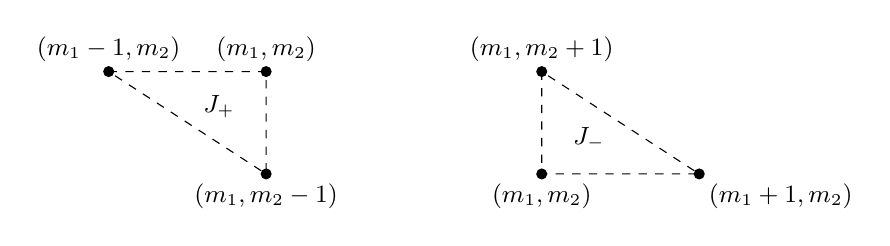
\begin{tikzpicture}[every node/.style={font=\small}]
  \fill (0,1.3) circle (2pt) node[above] {$(m_1-1,m_2)$};
  \fill (2,1.3) circle (2pt) node[above] {$(m_1,m_2)$};
  \fill (2,0) circle (2pt) node[below] {$(m_1,m_2-1)$};
  \draw[dashed] (0,1.3) -- (2,1.3) -- (2,0) -- cycle;
  \node at (1.4,0.85) {$J_+$};
  \begin{scope}[xshift=5.5cm]
    \fill (0,1.3) circle (2pt) node[above] {$(m_1,m_2+1)$};
    \fill (0,0) circle (2pt) node[below] {$(m_1,m_2)$};
    \fill (2,0) circle (2pt) node[below right] {$(m_1+1,m_2)$};
    \draw[dashed] (0,1.3) -- (0,0) -- (2,0) -- cycle;
    \node at (0.6,0.45) {$J_-$};
  \end{scope}
\end{tikzpicture}
\end{minipage}

neznáme jedno číslo $\forall j$ \\
$\to$ z normalizace a \kw{Condon--Shortley} konvence:
\[
  \braket{j_1j_2}{j_1+j_2,\,j_1+j_2} = 1, \qquad \braket{j_1,\,j-j_1}{j,j} > 0
\]

\textbf{SCHÉMA KONSTRUKCE:} \quad ($\forall j$ fixní $= j_1+j_2,\ j_1+j_2-1,\ \dots,\ 0$)

\begin{center}
\begin{tikzpicture}[defbarva,scale=0.85,every node/.style={font=\small}]
  % levý diagram
  \begin{scope}
    \fill[pattern=north east lines,pattern color=defbarva!60] (-2,-0.5) -- (-2,2) -- (0.5,2) -- (2,0.5) -- (2,-2) -- (-0.5,-2) -- cycle;
    \draw[->] (-3.4,0) -- (3.4,0) node[below] {$m_1$};
    \draw[->] (0,-3.2) -- (0,3.4) node[right] {$m_2$};
    \draw (-3.4,2) -- (3.2,2) node[above,pos=0.12] {$m_2 = j_2$};
    \draw (-3.4,-2) -- (3.2,-2) node[below,pos=0.12] {$m_2 = -j_2$};
    \draw (-2,-3.2) -- (-2,3.2);
    \node[left] at (-2,-0.4) {$-m_1 = j_1$};
    \draw (2,-3.2) -- (2,3.2);
    \node[right] at (2,-2.7) {$m_1 = j_1$};
    \draw (-0.8,3.3) -- (3.2,-0.7) node[below] {$m_1+m_2 = j$};
    \draw (-3.2,0.7) -- (0.8,-3.3) node[right] {$m_1+m_2 = -j$};
    \node[fill=white,fill opacity=0.8,text opacity=1,inner sep=1pt,align=center] at (-0.7,-0.3) {OBLAST\\ NENULOVÝCH\\ CG\\ (pro fix $j$)};
    \draw[prbarva,thick] (0.2,0.2) rectangle (2.6,2.6);
    \draw[prbarva,->,thick] (2.6,2.3) to[bend left=10] node[above] {Detail} (5.4,2.3);
  \end{scope}
  % detail
  \begin{scope}[xshift=6.3cm,yshift=-1.6cm,scale=0.95]
    \foreach \y in {0,1,2,3} \draw (-0.4,\y) -- (3.6,\y);
    \draw (0,-0.6) -- (0,4.4);
    \draw (1,-0.6) -- (1,3.6);
    \draw[very thick] (2,-0.6) -- (2,3);
    \draw (-0.2,4.5) -- (1,3) -- (2.9,1.1);
    \foreach \x/\y in {0/4,0/3,0/2,0/0,1/3,1/2,1/1,1/0,2/2,2/1,2/0} \fill (\x,\y) circle (2.5pt);
    \draw (0,1) circle (2.5pt);
    \foreach \x/\y in {3.3/2,3.3/1,3.3/0,2/3.3} \node at (\x,\y) {$0$};
    \node[right] at (2.6,3.6) {CG $= 0$};
    \node[above right] at (2,2) {A \dots\ zvolím};
    \node[above left] at (1,2) {C};
    \node[below left] at (1,1) {D};
    \node[below right] at (2,1) {B};
    \node[below right] at (2,0) {E};
    \begin{scope}[prbarva,thick]
      \draw (1.1,1.9) -- (1.9,1.9) -- (1.9,1.1) -- cycle;
      \node at (1.65,1.65) {\scriptsize $J_+$};
      \draw (1.1,1.85) -- (1.1,1.1) -- (1.85,1.1) -- cycle;
      \node at (1.35,1.35) {\scriptsize $J_-$};
      \draw (2.1,1.9) -- (2.1,1.1) -- (2.9,1.1) -- cycle;
      \node at (2.35,1.35) {\scriptsize $J_\mp$};
      \draw (1.1,0.9) -- (1.9,0.9) -- (1.9,0.1) -- cycle;
      \node at (1.65,0.65) {\scriptsize $J_+$};
    \end{scope}
    \foreach \y in {-0.4,0.6,1.6} \draw[defbarva!60] (-0.3,\y) -- (0.8,\y+1.1);
  \end{scope}
\end{tikzpicture}
\end{center}
\hfill postupná konstrukce z A, např.\ v pořadí ABCDE \dots

\begin{priklad}[PŘÍKLAD: částice se spinem $\frac12$ ve sfér.\ poli, $\hat{\vec L}$ komutuje s $H$]
$\mathcal{H} = \mathcal{H}_{\text{orbit}}\otimes\mathcal{H}_{\text{spin}}$ \qquad $\hat{\vec J} = \hat{\vec L} + \hat{\vec S}$

\dots\ tj.\ \quad
$\begin{aligned} j_1 &= l & m_1 &= m_l \\ j_2 &= s = \tfrac12 & m_2 &= m_s = \pm\tfrac12 \end{aligned}$
\qquad $\Delta$-nerovnost povoluje jen $j = l\pm\frac12$ \\
\hspace*{11.2cm} (pro $l = 0$ jen $j = \frac12$)
\end{priklad}

%----------------------------------------------------------------------
\strana{AA-6}
\subsubsection*{Konstrukce C-G pro $\vec J = \vec L + \vec S$:}

\begin{center}
\begin{tikzpicture}[defbarva,x=0.9cm,y=1cm,every node/.style={font=\small}]
  \draw[->] (-4.5,0) -- (7,0) node[right] {$m_l$};
  \draw[->] (0,-1) -- (0,1.2) node[right] {$m_s$};
  \node at (-4.8,0.5) {$+\frac12$};
  \node at (-4.8,-0.5) {$-\frac12$};
  % řádek +1/2
  \foreach \x in {-3.5,-2} \draw (\x,0.5) circle (2pt);
  \foreach \x in {0,1,2,3,4} \fill (\x,0.5) circle (2.5pt);
  % řádek -1/2
  \foreach \x in {-3.5,-2} \draw (\x,-0.5) circle (2pt);
  \foreach \x in {0,1,2,3,4} \fill (\x,-0.5) circle (2.5pt);
  % nuly nad
  \foreach \x in {2,3,4} \draw (\x,1.2) circle (2pt);
  \node[right] at (4.6,0.45) {$\leftarrow m_s = \frac12$};
  \node[above right] at (4,0) {$+l$};
  % diagonály
  \draw (1.2,1) -- (3.3,-1.1) node[below left] {$j$};
  \draw (2.2,1) -- (4.2,-1) node[below] {$j = l-\frac12$};
  \draw (3.3,1.2) -- (5.4,-1) node[below right] {$j = l+\frac12$};
  % J- trojúhelníky
  \begin{scope}[prbarva,thick]
    \draw (2,1.2) -- (2,0.5) -- (3,0.5) -- cycle; \node at (2.3,0.75) {\scriptsize $J_-$};
    \draw (3,1.2) -- (3,0.5) -- (4,0.5) -- cycle; \node at (3.3,0.75) {\scriptsize $J_-$};
  \end{scope}
\end{tikzpicture}
\end{center}

pro $j = l + \frac12$ \ ($R_-$):
\begin{multline*}
  \sqrt{\big(l+\tfrac12+m+1\big)\big(l+\tfrac12-m\big)}\,\braket{m-\tfrac12,\tfrac12}{l+\tfrac12,m} \\
  = \sqrt{\big(l+m+\tfrac12\big)\big(l-m+\tfrac12\big)}\,\braket{m+\tfrac12,\tfrac12}{l+\tfrac12,m+1}
\end{multline*}
\hspace*{7.5cm} $\nwarrow$ pro $m = l+\frac12,\ l-\frac12,\ \dots,\ -l-\frac12$

přičemž konvence diktuje $\braket{l,\tfrac12}{l+\tfrac12,\,l+\tfrac12} = 1$ \\
$\to$ iterace
\begin{align*}
  &\braket{m-\tfrac12,\tfrac12}{l+\tfrac12,m} \\
  &\quad= \sqrt{\frac{(l+m+\frac12)\,{\color{gray}(l-m+\frac12)}}{(l+m+\frac32)\,{\color{gray}(l-m+\frac12)}}}\ \braket{m+\tfrac12,\tfrac12}{l+\tfrac12,m+1}
     \quad \pozn{krácení} \\
  &\quad= \sqrt{\frac{l+m+\frac12}{l+m+\frac32}}\sqrt{\frac{l+m+\frac32}{l+m+\frac52}}\ \braket{m+\tfrac32,\tfrac12}{l+\tfrac12,m+2}
     \quad \pozn{$m\to m+1$} \\
  &\quad\ \ \vdots \\
  &\quad= \sqrt{\frac{l+m+\frac12}{2l+1}}\ \underbrace{\braket{l,\tfrac12}{l+\tfrac12,\,l+\tfrac12}}_{=1}
\end{align*}
tj.\ \quad
$\vzorec{\braket{m-\tfrac12,\tfrac12}{l+\tfrac12,m} = \sqrt{\frac{l+m+\frac12}{2l+1}}}$
\quad \dots\ jen horní řádek pro $j = \frac12 + l$; \\
\hspace*{8.6cm} ještě dolní řádek a hodně $j = l - \frac12$

C-G matice je blok.\ diagonální \dots\ nenulové jen bloky $m = m_1 + m_2$ \quad $\swarrow$ matice pro fixní $l, s$

\begin{minipage}{0.5\textwidth}
\begin{tikzpicture}[scale=0.85,every node/.style={font=\scriptsize}]
  \draw (-0.2,2.2) to[bend right=15] (-0.2,-1.2);
  \draw (4.6,2.2) to[bend left=15] (4.6,-1.2);
  \draw (0,1.2) -- (4.4,1.2) (0,0) -- (4.4,0);
  \draw (1.8,2.4) -- (1.8,-1.4) (3.1,2.4) -- (3.1,-1.4);
  \node at (2.45,0.9) {$\cos\phi\ \ \sin\phi$};
  \node at (2.45,0.35) {$-\sin\phi\ \ \cos\phi$};
  \node[defbarva,above] at (2.45,2.4) {$j = l+\frac12,\ l-\frac12$};
  \draw[defbarva,->,thick] (2.3,2.4) -- (2.3,1.6);
  \node[left,align=right] at (-0.2,0.6) {$m_l\,m_s$\quad $m-\frac12,\ +\frac12$\\ $m+\frac12,\ -\frac12$};
  \draw[defbarva,->,thick] (0,0.9) -- (1.6,0.9);
  \draw[decorate,decoration={brace,amplitude=3pt}] (4.7,1.2) -- (4.7,0) node[midway,right=3pt] {blok $m$};
  \draw[decorate,decoration={brace,mirror,amplitude=3pt}] (1.8,-1.5) -- (3.1,-1.5) node[midway,below=3pt] {blok $m$};
\end{tikzpicture}
\end{minipage}
\begin{minipage}{0.46\textwidth}
\dots\ + \fcolorbox{defbarva}{white}{UNITARITA}
\[
  \cos\phi = \sqrt{\frac{l+m+\frac12}{2l+1}}
\]
\begin{align*}
  \sin\phi &= \sqrt{1-\cos^2\phi} \\
  &= \sqrt{\frac{l-m+\frac12}{2l+1}} = \braket{m-\tfrac12,\tfrac12}{\ }
\end{align*}
\end{minipage}

\noindent\rule{\linewidth}{0.4pt}

\begin{definice}[spin-úhlové funkce \pozn{spin-orbitaly}]
\begin{align*}
  \mathcal{Y}_l^{\,j=l\pm\frac12,m}
  &= \pm\sqrt{\frac{l\pm m+\frac12}{2l+1}}\,Y_l^{m-\frac12}(\theta,\varphi)\,\chi_+
     + \sqrt{\frac{l\mp m+\frac12}{2l+1}}\,Y_l^{m+\frac12}(\theta,\varphi)\,\chi_- \\
  &= \frac{1}{\sqrt{2l+1}}\begin{pmatrix} \pm\sqrt{l\pm m+\frac12}\ Y_l^{m-1/2}(\theta,\varphi) \\ \sqrt{l\mp m+\frac12}\ Y_l^{m+1/2}(\theta,\varphi)\end{pmatrix}
  \qquad\dots\ \text{vlast.\ fce } L^2, S^2, J^2 \text{ a } J_z
\end{align*}
\end{definice}

$\Rightarrow$ také vl.\ fce \quad
$\vec L\cdot\vec S = \frac12\big(J^2 - L^2 - S^2\big) = \frac{\hbar^2}{2}\Big(j(j+1) - l(l+1) - \frac34\Big)$
$\begin{cases}
  \oplus:\ \ \frac{l}{2}\hbar^2 & \text{pro } j = l+\frac12 \\[2pt]
  \ominus:\ -\frac{l+1}{2}\hbar^2 & j = l-\frac12
\end{cases}$

